\pagestyle{ayllon}
\label{ayllon}


\pagebreak
\begin{center}
\hspace*{-3.6cm}\raisebox{5cm}{\rotatebox[origin=t]{90}{\huge\textbf{Lançamento}}}
\hspace*{3.1cm}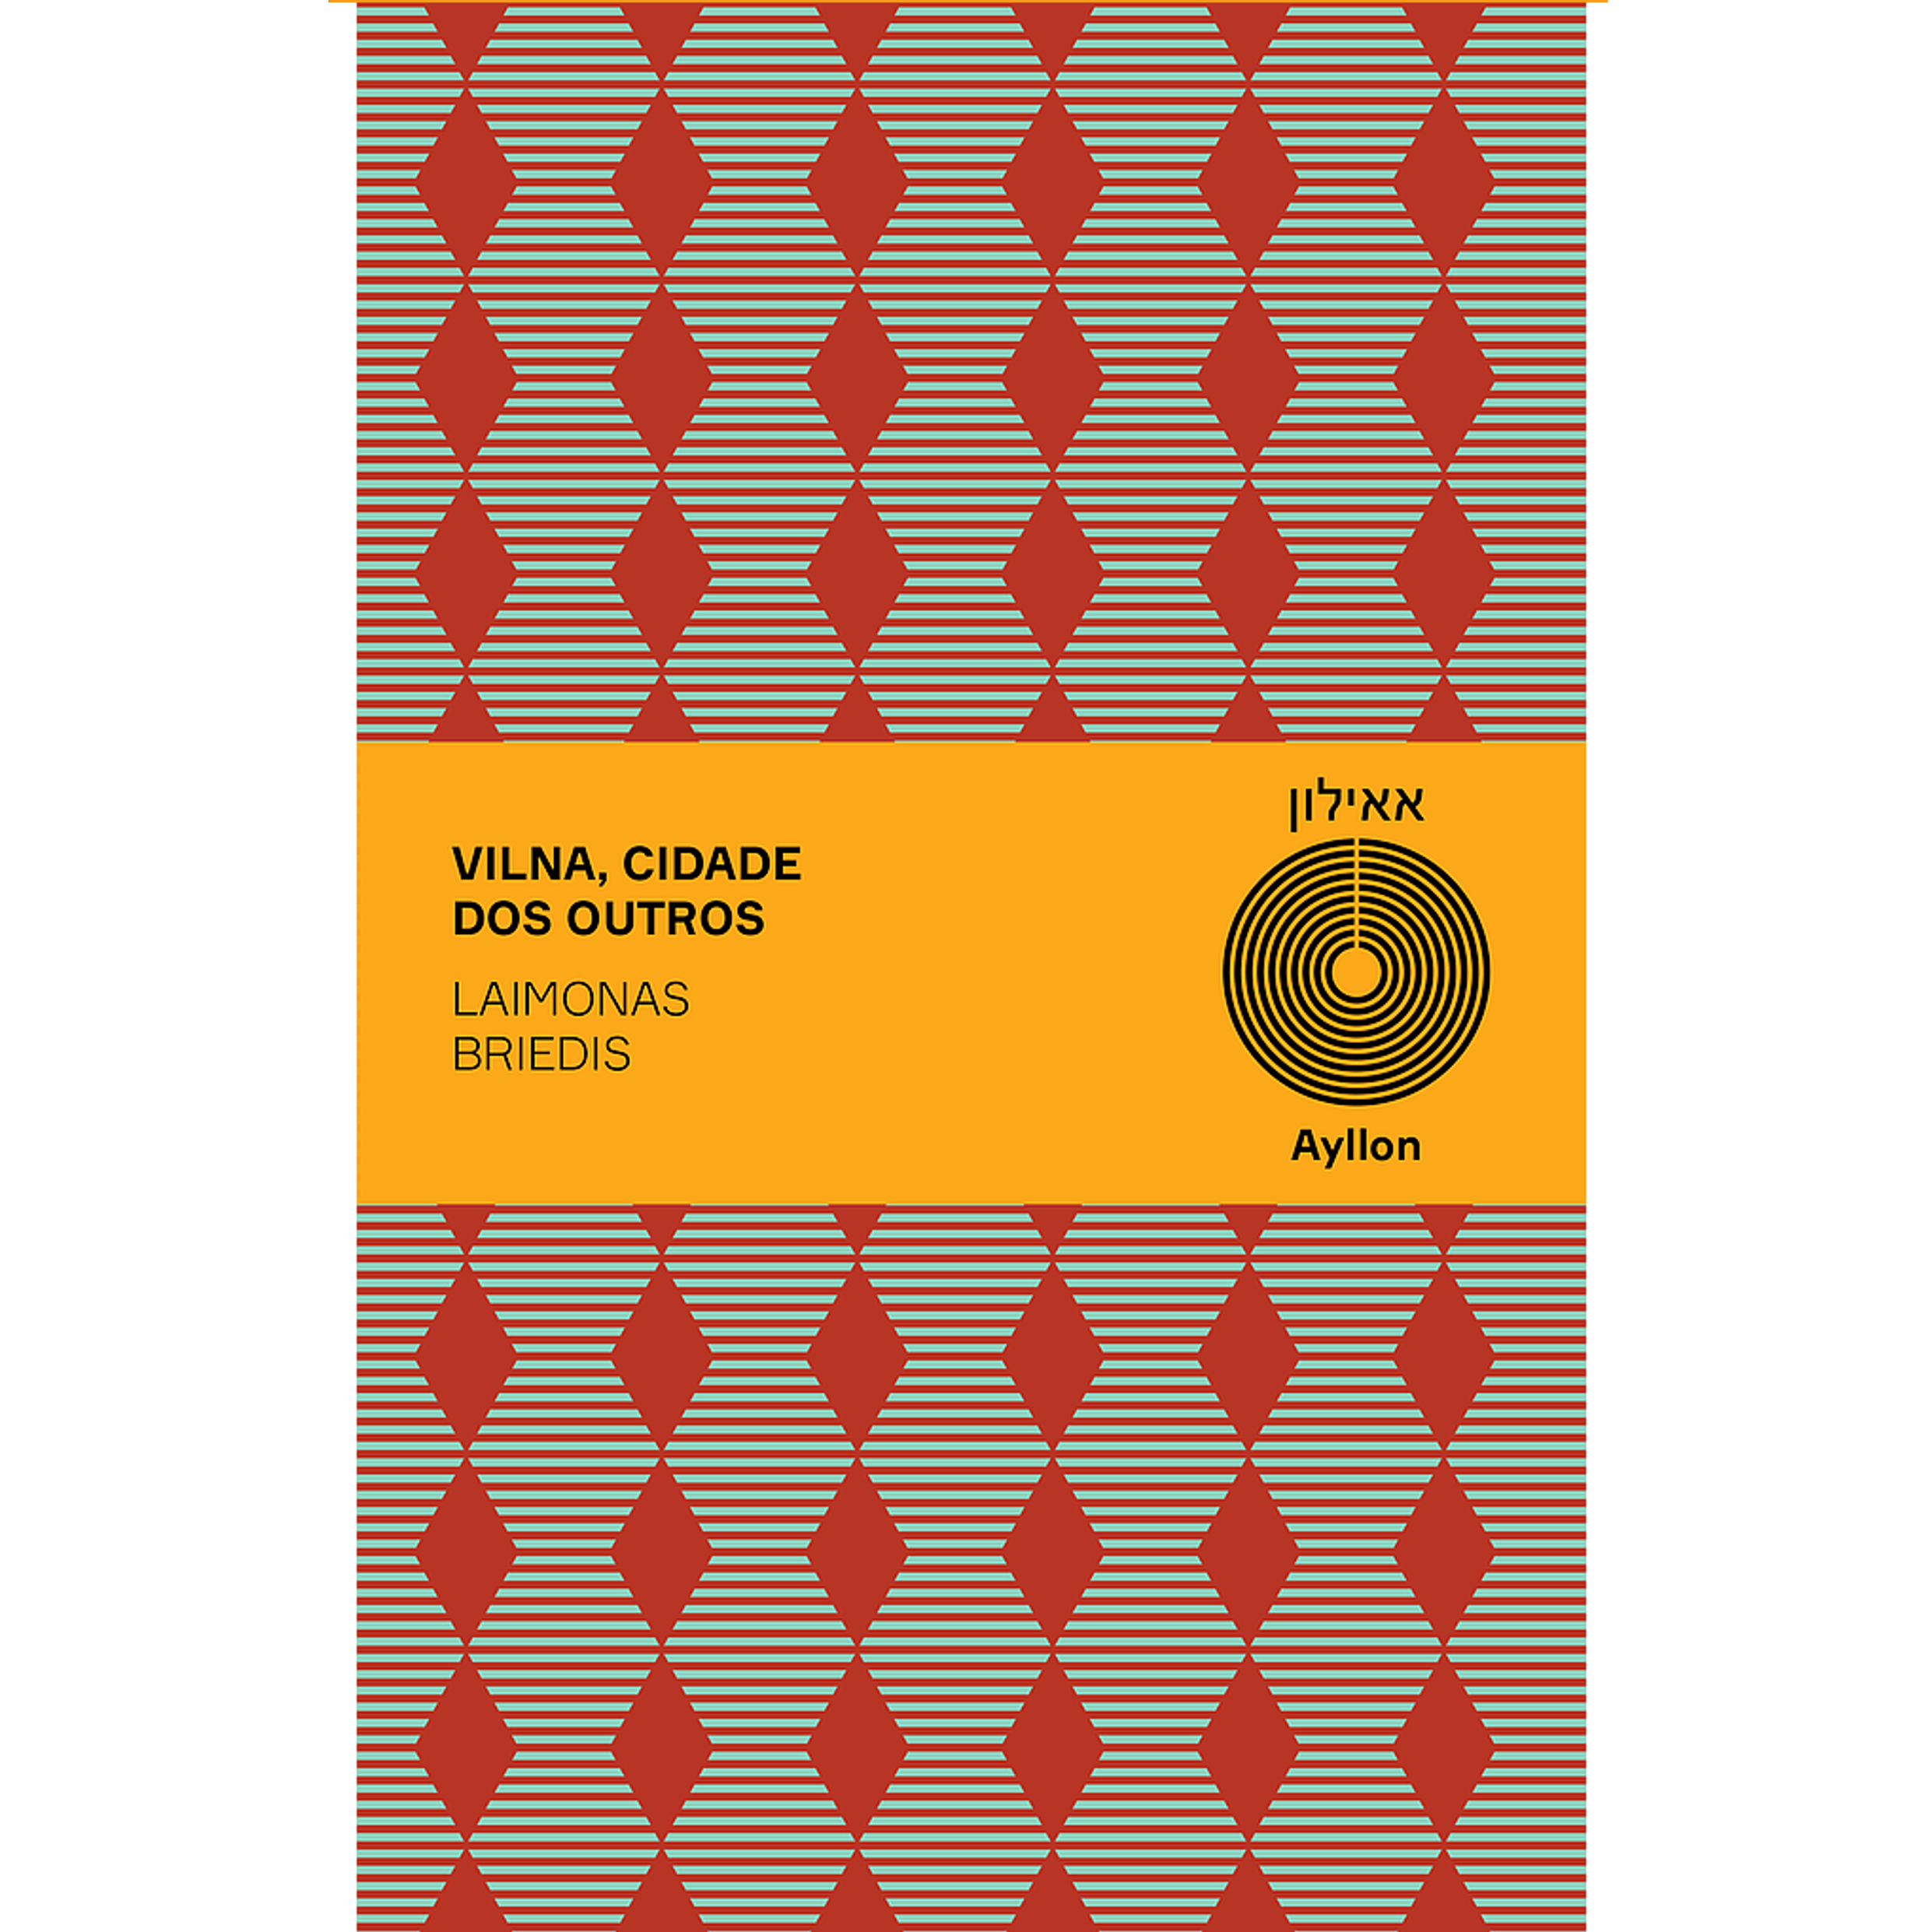
\includegraphics[width=74mm]{./CAPAS/AYLLON_VILNA.jpg}
\end{center}
\hspace*{-7cm}\hrulefill\hspace*{-7cm}
\medskip

\noindent{}\textit{Vilna, cidade dos outros} é uma narrativa sobre a capital da Lituânia. \hlc{Escrita com base na cartografia histórica e geografia humana local, a cidade que também foi conhecida como "a Jerusalém da Lituânia" abrigou ao longo dos tempos inúmeros povos, falantes de diversos idiomas, em uma miscelânia cultural: judeus, poloneses, lituanos, ucranianos, bielorussos, russos, alemães, letões, armênios, tártaros} e outros grupos minoritários. Impregnada dentre seus vários componentes pelo barroco, que esteve no limiar da Europa e no contexto de suas mudanças, a cosmopolita cidade também é apresentada através de textos de pessoas ilustres ou desconhecidas, de muitas procedências e línguas, que viveram ou passaram por ela, através de relatos de experiências, sensibilidades e perspectivas próprias.

\vfill
\hspace*{-.4cm}\begin{minipage}[c]{1\linewidth}
\small\textbf{
\hspace*{-.1cm}Editora: Ayllon\\
Título: Vilna, cidade dos outros\\
Autor: Laimonas Briedis\\ 
ISBN: 978-85-77156-65-8\\
Páginas: 380\\
Formato: 13,3x21\,cm\\
Preço: R\$ 99,00
}
\end{minipage}
\pagebreak

\begin{center}
\hspace*{.5cm}
\includegraphics[width=74mm]{./CAPAS/AYLLON_BLECHER.jpg}
\end{center}
\hspace*{-7cm}\hrulefill\hspace*{-7cm}
\medskip

\noindent{}\textit{Acontecimentos na irrealidade imediata} foi originalmente publicado em 1936, e é composto por um \hlc{amálgama caleidoscópico de situações que cruzam o caminho do narrador, um personagem desajustado ao mundo.} Esses􏰃􏰀 acontecimentos arrastam-no a um turbilhão de pensamentos e ações atravessados por forças contrapostas, no qual as percepções misturadas da realidade, do tempo e do espaço dão lugar a um tipo diferente de discurso, que oferece inquietações fragmentadas ao invés de uma ordem racional.

\vfill
\noindent\begin{minipage}[c]{1\linewidth}
{\small\textbf{
\hspace*{-.1cm}Editora: Ayllon\\
Título: Acontecimentos na irrealidade imediata\\
Autor: Max Blecher\\ 
ISBN: 978-65-89705-07-9\\
Páginas: 170\\
Formato: 13,3x21\,cm\\
Preço: R\$ 54,00\\
}}
\end{minipage}
\pagebreak

\begin{center}
\hspace*{-3.6cm}\raisebox{5cm}{\rotatebox[origin=t]{90}{\huge\textbf{Lançamento}}}
\hspace*{3.1cm}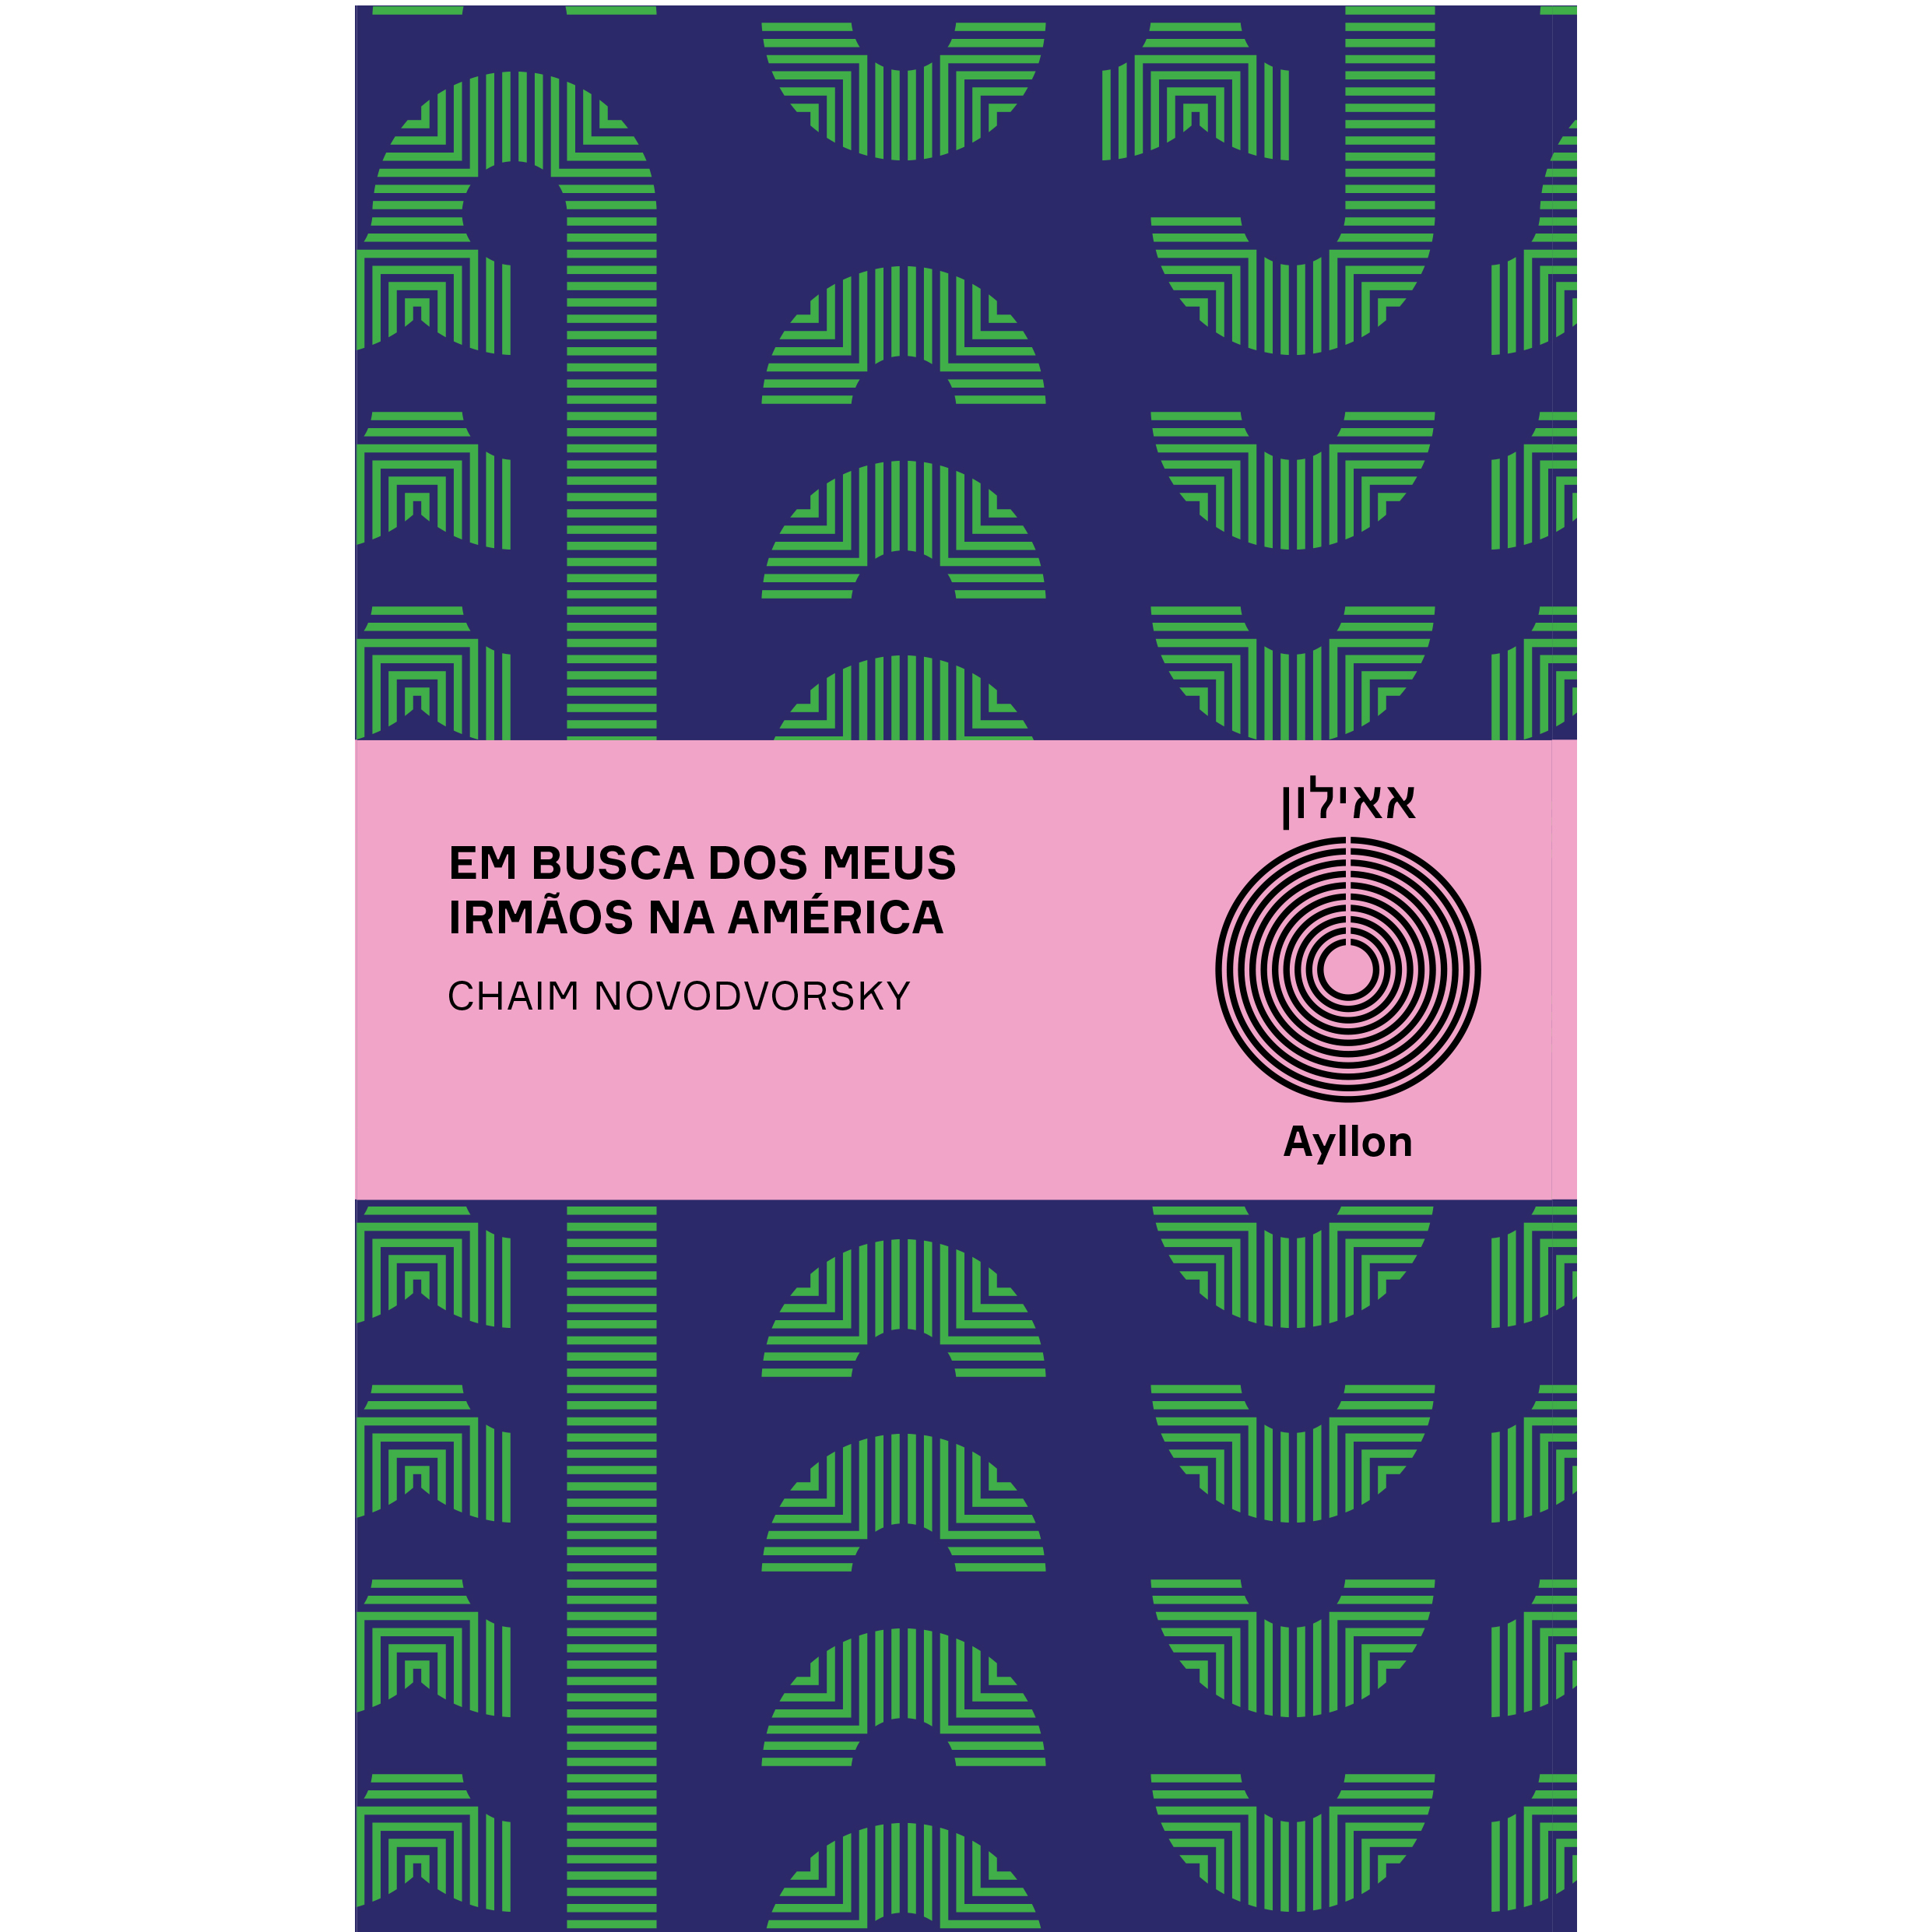
\includegraphics[width=74mm]{./CAPAS/AYLLON_AMERICA.jpg}
\end{center}
\hspace*{-7cm}\hrulefill\hspace*{-7cm}
\medskip

\noindent{}\textit{Em busca de meus irmãos na América}, de Chaim Novodvorsky, é um texto de memória que prende o leitor do começo ao fim. \hlc{É um relato pessoal, singular, e, ao mesmo tempo, emblemático dos percursos da imigração judaica. Mescla de forma saborosa os acontecimentos e as aventuras pessoais} de um imigrante polonês que foi primeiro à Argentina, depois ao Uruguai e, finalmente, ao Brasil, com um preciso e vívido retrato dos caminhos pelos quais se dava a inserção dos imigrantes na vida do país entre os anos 1920 e 1960. 

\vfill
\noindent\begin{minipage}[c]{1\linewidth}
{\small\textbf{
\hspace*{-.1cm}Editora: Ayllon\\
Título: Em busca de meus irmãos na América\\
Autor: Chaim Novodvorsky\\ 
ISBN: 978-65-89705-29-1\\
Páginas: 99 (provisório)\\
Formato: 13,3x21\,cm\\
Preço: R\$ 43,00\\
}}
\end{minipage}
\pagebreak

\vspace*{1.5cm}
\noindent{}{\nohyphens{\LARGE{A Jerusalém da Lituânia}}}
\bigskip

\hfill{}\scalebox{.8}{CELSO LAFER}
\bigskip
\bigskip
\bigskip

\begin{multicols}{2}

% {\small\fakereceipt{
% \noindent{}\lipsum[7]
% }}
% \vspace{\baselineskip}

\noindent{}\textit{\textit{Vilnius}} é hoje a capital da Lituânia. O fim da União Soviética e as transformações econômicas e políticas, que dela derivaram, assinalaram o término das relevâncias geopolíticas da Europa Oriental como um componente da Guerra Fria. Nessa nova moldura, a Lituânia tornou"-se um país independente, dotado de autonomia na condução de sua política e na gestão de seus assuntos internos. É uma cidade demograficamente lituana e de fala lituana.

Esta é, no entanto, uma nova realidade no percurso histórico de uma
cidade muito impregnada, em seus componentes medievais, pelo barroco,
que viveu no limiar da Europa e no contexto de suas mudanças
cartográficas, e cujos habitantes de diversas origens, por isso mesmo,
percorreram suas casas e ruas, falando, sucessiva ou concomitantemente,
várias línguas. Articularam, assim, em diversos idiomas, suas vivências
e memórias.

A cidade foi por isso mesmo um \textit{locus} paradigmático da
\textit{heteroglossia}, termo cunhado e teoricamente elaborado pelo grande
crítico russo Mikhail Bakhtin. Bakhtin viveu sua juventude em Vilna, de
1904 a 1912, quando seu pai integrava a administração russa da cidade.
Provavelmente, inspirou"-se em sua vivência ali, como sugere Laimonas
Briedis, para a elaboração teórica a respeito das correlações temporais
e espaciais de vários âmbitos linguísticos.

\textit{\textit{Vilnius}} foi \textit{Vilna}, denominação em eslavo, que assinala a longa
eslava presença no tempo na cidade da Rússia tzarista e soviética.
Também foi \textit{Wilno} para os poloneses, o que realça o histórico
relacionamento da Lituânia e da Polônia, que está na origem política dos
dois países. Também foi \textit{Wilna} para os alemães, que tiveram relevantes
passagens nas incursões da Alemanha no Leste Europeu pela cidade. Para
os judeus \textit{ashkenazim}, foi, em iídiche, \textit{Vilnè}, a irradiadora
\textit{Jerusalém da Lituânia} no mundo judaico, identificadora das
características culturais e religiosas de seus \textit{litvaks}, que,
dizimados pelo Holocausto, desapareceram da cidade.

Esta problematicidade se revela no título do livro de Laimonas Briedis,
no original inglês, \textit{Vilnius, City of Strangers}, e na tradução
para o português, \textit{Vilna, cidade dos outros}, que se deve aos
cuidados de Fernando Klabin e, ao optar pela forma ``Vilna'', ecoa o nome
da cidade no final do século \textsc{xix}, quando a família Klabin imigrou da
Lituânia e encontrou seu destino no Brasil.

Czeslaw Miłosz, grande poeta da língua polonesa, prêmio Nobel de
Literatura que nasceu na Lituânia e estudou em Vilna, intitula, não por
acaso, um de seus poemas ``Cidade sem nome'', que começa indagando
``Quem honrará a cidade sem nome/\,se tantos estão mortos\dots{}''\footnote{Czeslaw Miłosz. \textit{Selected and Last Poems --
  1931--2004}. Seleta de Robert Hass e Anthony Miłosz. Nova York: Harper
  Collins; Ecco Paperback Edition, 2011, p. 261. Na edição original, o poema é grafado ``City without a name'': ``Who will honor the city without a name/\,if so many are
dead\ldots{}''.}

Os diversos grupos étnicos que assinalaram, no correr dos tempos, a
composição demográfica da cidade, articularam, em suas respectivas
línguas, sua compreensão histórica do que é hoje \textit{Vilnius}. Foi o que
induziu Laimonas Briedis a escrever \textit{Cartografia poética:
 Bobrowski, Miłosz, Sutzkever}, publicado em 2015.\footnote{Laimonas Briedis.
  \textit{Poetic Cartography: Bobrowski, Miłosz, Sutzkever}. \textit{Vilnius}: \textit{Vilnius} University, 2015.} Nele examina
o papel da cidade como fonte inspiradora da criação poética de Bobrowski, escritor de língua alemã que não viveu em \textit{Vilnius}, mas a cidade é
parte do simbolismo que a ela atribuiu na História e na Geografia da
Europa Oriental. De Miłosz -- que já mencionei --, poeta da língua
polonesa, que experienciou o exílio, iniciado quando jovem deixou a
Lituânia. E de Sutzkever, poeta da língua iídiche, que viveu no gueto de
Vilna a presença nazista na cidade. As biografias e a poesia dos três
são muito distintas, mas a cidade integra suas destilações poéticas. Na
avaliação de Laimonas Briedis, para Miłosz, \textit{Vilnius} é um local de
memória da normalidade de vida; para Bobrowski, o local das não
realizadas possibilidades da normalidade de vida; para Sutzkever, o
local das anormalidades de vida.\footnote{\textit{Idem, ibid.}, p. 89.}

\vspace{\baselineskip}
{\small\fakereceipt{
\noindent{}São os itinerários dos caminhantes que passaram ou viveram em \textit{Vilnius}
que nortearam, com sensibilidade europeia, o ``sair em visita'' de
Laimonas Briedis na construção de sua narrativa.}}
\vspace{\baselineskip}

Em todos os três, a experiência de base da perda e da dor provém do fato
de que as rupturas do século \textsc{xx} fizeram, como analisou Hannah Arendt,
com que a política determinasse, independentemente de suas vontades, os
rumos de vida, como, aliás, para tantas pessoas na Europa. Os três foram, assim, 
para Laimonas Briedis, uma chave para a
compreensão da complexidade de uma cidade que ele não vivenciou e que
não tem uma identidade de fácil ou inequívoca definição.

Hannah Arendt destacou em sua obra, a partir de sua experiência
reflexiva a respeito das rupturas inerentes aos extremos do século \textsc{xx}, o
poder redentor e esclarecedor da narrativa.

Numa época de ``universais fugidios'', a narrativa, em conjunto com a
pluralidade e a natalidade, configura as facetas constitutivas da ação
humana. No curso que com ela fiz, em 1965, na Universidade de Cornell, e
em outros escritos, Arendt deu ênfase ao que Kant denominou a
``mentalidade alargada'', que permite pensar no lugar de outros. Isso
requer um tipo de imaginação que enseja levar em conta a perspectiva dos
outros e de suas circunstâncias. É um \textit{go visiting}, ``sair em
visita'', que torna presente o ponto de vista dos que estão
ausentes.\footnote{Celso Lafer, ``Experiência, ação e narrativa:
  reflexão sobre um curso de Hannah Arendt''. Em \textit{Hannah Arendt:
  pensamento, persuasão e poder}. Rio de Janeiro:
  Paz e Terra, 2018, pp. 51--73.}

% Faço esta remissão a Hannah Arendt porque ela contribui para destacar o
% mérito e a amplitude com a qual Laimonas Briedis ``saiu em visita'' para
% elaborar o juízo reflexivo de sua narrativa do percurso no tempo da
% cidade de \textit{Vilnius} e da multiplicidade de perspectivas dos que nela
% viveram.

George Steiner, ao escrever sobre \textit{A ideia de Europa}\footnote{George Steiner, 
\textit{A ideia de Europa}. Lisboa: Relógio d'Água, 
2017, pp. 30--32.}, aponta que
são elementos do pensamento e da sensibilidade europeia a ordem e a
cadência de seus caminhantes em seus diversificados itinerários no
espaço de sua região.

São os itinerários dos caminhantes que passaram ou viveram em \textit{Vilnius}
que nortearam, com sensibilidade europeia, o ``sair em visita'' de
Laimonas Briedis na construção de sua narrativa.

A narrativa de Laimonas Briedis é um tecido de qualidade literária, que
entrelaça com originalidade a trama e o urdume. O ``urdume'' explica as
grandes forças políticas e movimentos demográficos que situaram a
Lituânia, desde suas origens, no limiar da Europa e suas vicissitudes. O
autor desvenda"-as pelo sagaz uso da cartografia e de suas dimensões
históricas com um acurado conhecimento da geografia humana. É muito
instigante o uso que sabe fazer dos mapas. A ``trama'' revela os nexos de
sentido da compreensão transversal dos fios da vida inserida no correr
dos séculos no urdume. O autor ilumina esses nexos de sentido pelos
relatos de pessoas de distintas procedências que viveram ou passaram
pela cidade e que escreveram em mais de uma língua sobre suas
experiências na cidade, a partir de suas sensibilidades e perspectivas.
A escolha desses relatos é fruto de uma garimpagem literária e cultural
de sensibilidade e abertura que deslinda o alcance geral da
particularidade de Vilna. Daí a \textit{vis atractiva} desta obra que se
insere no patamar de qualidade do gênero literário de livros sobre
cidades. Em síntese, Laimonas Briedis soube nomear e honrar, para evocar
novamente o poema de Miłosz, ``[\ldots{}] cidade sem nome/\,se tantos estão mortos''.

\bigskip
\noindent{}\textcolor{gray}{\footnotesize\slsc{\textls[-15]{Adaptação de excerto do prefácio de ``Vilna: cidade dos outros''.}}}
\end{multicols}

\pagebreak
\pagestyle{aylloncat}
\begin{multicols}{2}
\begin{enumerate}
\raggedright\nohyphens{
\item Yitzhak Rabin: uma biografia \textbf{Itamar Rabinovich; Samuel Feldberg; Debora Fleck}
\item Fragmentos de um diário encontrado \textbf{Mihail Sebastian; Fernando Klabin; Luis Krausz; Gabriel Neinstein}
\item Cabalat shabat: poemas rituais \textbf{Fabiana Gampel Grinberg}
\item Israel e Palestina \textbf{Gershon Baskin; Christian Dunker}
\item Vilna: cidade dos outros \textbf{Laimonas Briedis; Fernando Klabin; Celso Lafer}
}
\end{enumerate}
\end{multicols}
\pagebreak